\chapter{Results} \label{chap:results}

In this chapter, we will test the selected models on the testing dataset, which contains 300 real images acquired by AGO70. First, we will test the model trained on the synthetic data from the Section \ref{subsec:finalmodel}. Next, we will test the models that were fine-tuned using real data in the training process. We proposed two approaches and have therefore two different models (Sections \ref{subsec:mergedmodel}, \ref{subsec:fcmodel}), which will be both tested separately. Finally, we will compare the performance of our models to the pre-trained ResNet-18 model. 

To measure the performance of our model we are using the following metrics: 
\begin{equation}
    Accuracy = \frac{TP + TN}{TP + FP + TN + FN}
\end{equation} 
\begin{equation}
    Recall = \frac{TP}{TP + FN}
\end{equation}
\begin{equation}
    Precision = \frac{TP}{TP + FP}
\end{equation}
where TP are true positives, FP are false positives, TN are true negatives and FN are false negatives. 

\section{Model trained on the synthetic data}

The final model from Section \ref{subsec:finalmodel} was evaluated on the testing dataset and has achieved 73.00 \% accuracy, 73.52 \% precision and 73.00 \% recall. 

From the confusion matrix in the Figure \ref{img:confmatrixsyn} we can see that the model has the biggest problem distinguishing between galaxy and streak (more than 30 cases). This is caused by the fact that elliptical galaxies with a high degree of ellipticity resemble streaks and even professionals wouldn't be able to tell the difference just from one image. Another prevalent problem is the misclassification of streaks as points (10 cases) and points as cosmic rays (13 cases). In the Figure \ref{fig:wrongsyn} we show some examples of wrongly classified images, where we can see that these problems are usually caused by small streaks that resembled points (\ref{fig:streakpointmis3}), and points with small fwhm which caused them to look like spots (\ref{fig:pointcosmicmis3}).   

\begin{figure}[h]
    \centering
    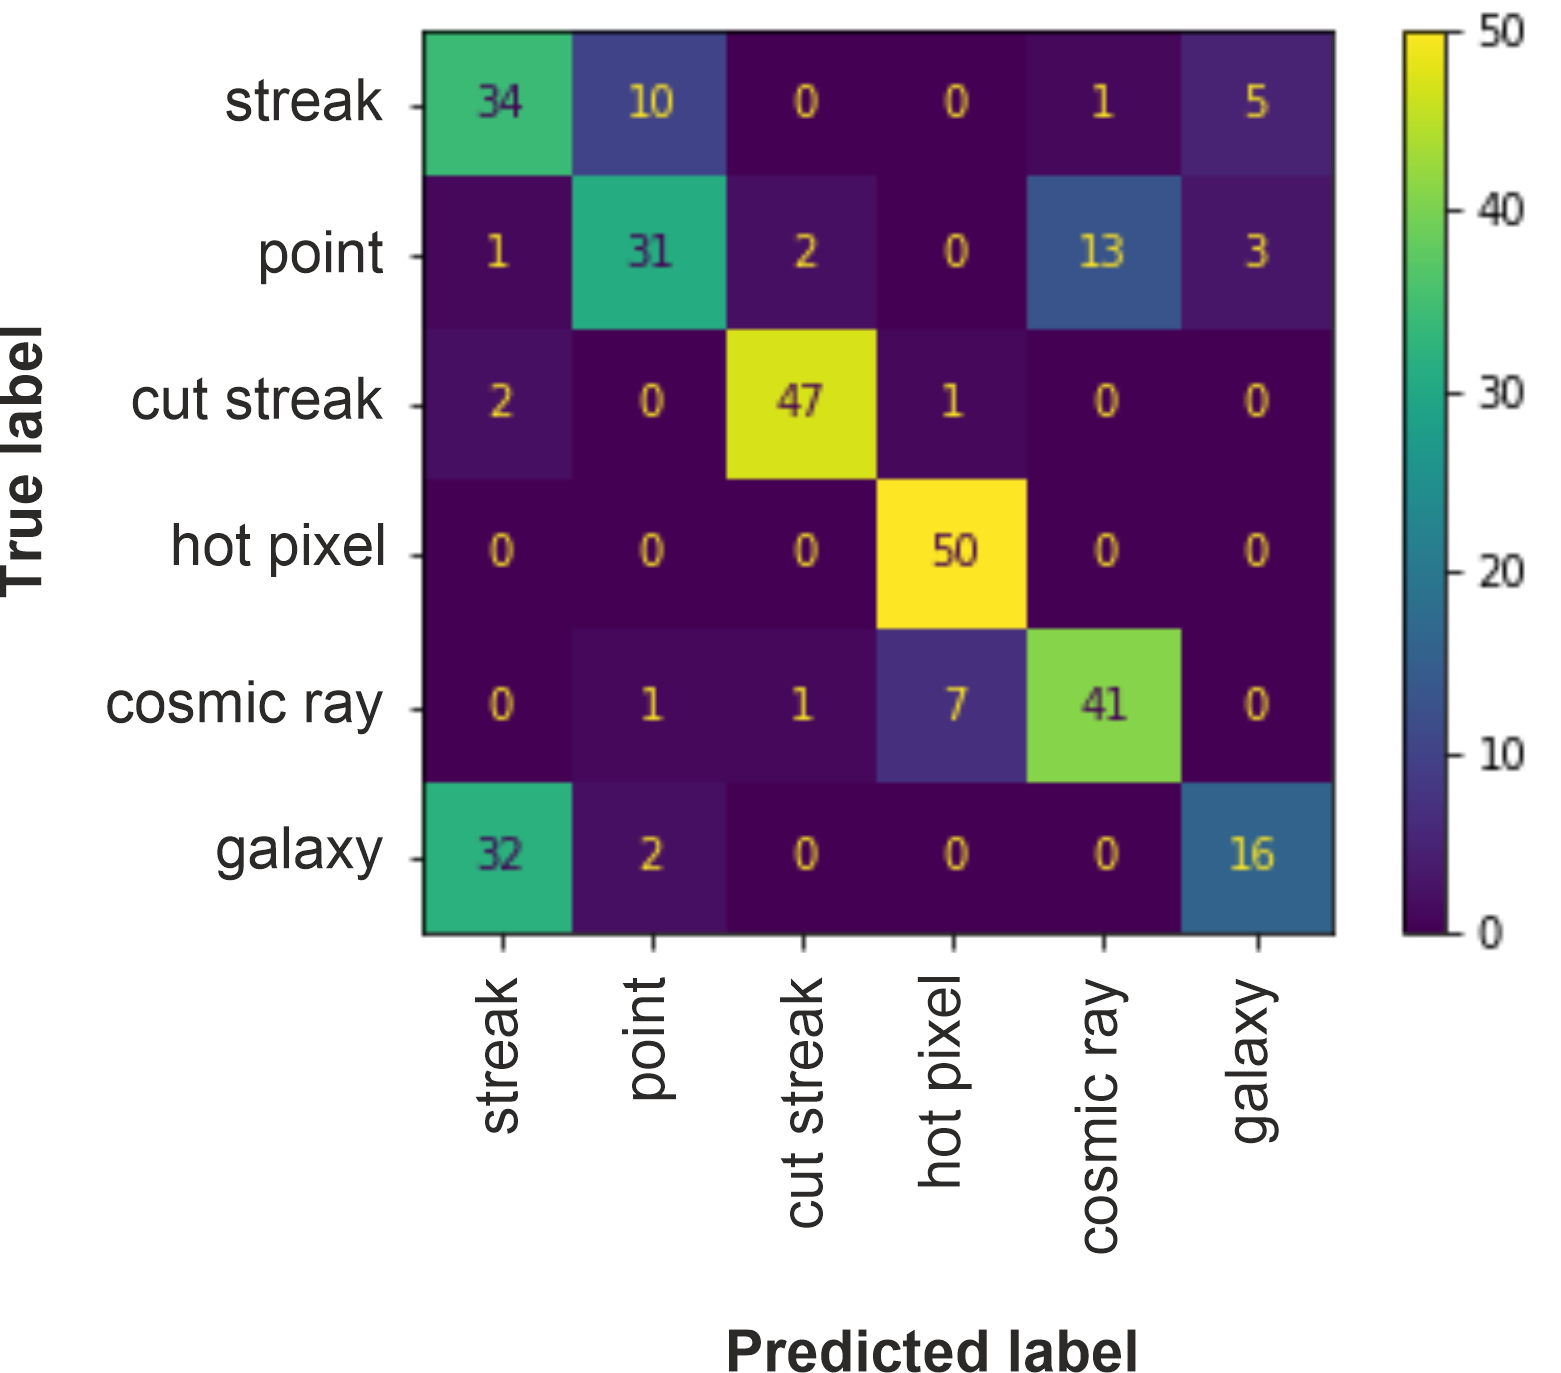
\includegraphics[width=.5\textwidth]{images/confusionmatrix51.png}
    \caption{Confusion matrix from the testing of the final model trained only on synthetic data.}
    \label{img:confmatrixsyn}
\end{figure}

\begin{figure}[!h]
\centering
    \begin{subfigure}[t]{.23\textwidth}
        \centering
        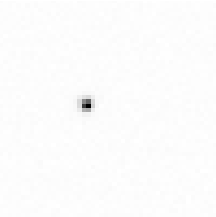
\includegraphics[width=\textwidth]{images/wrongImage8.png}
        \caption{}
        \label{fig:pointcosmicmis3}
    \end{subfigure}
    \begin{subfigure}[t]{.23\textwidth}
        \centering
        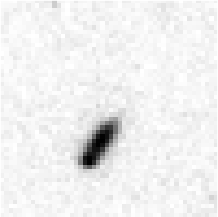
\includegraphics[width=\textwidth]{images/wrongImage18.png}
        \caption{}
    \end{subfigure}
    \begin{subfigure}[t]{.23\textwidth}
        \centering
        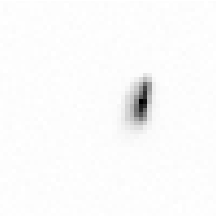
\includegraphics[width=\textwidth]{images/wrongImage34.png}
        \caption{}
    \end{subfigure}
    \begin{subfigure}[t]{.23\textwidth}
        \centering
        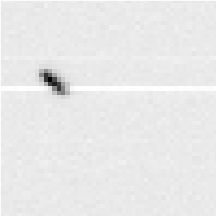
\includegraphics[width=\textwidth]{images/wrongImage48.png}
        \caption{}
        \label{fig:streakpointmis3}
    \end{subfigure}

    \caption[Wrongly classified images on the model that trained only with synthetic data.]{Wrongly classified images on the model that trained only with synthetic data. (a) A point misclassified as a cosmic ray, (b) A galaxy misclassified as a streak, (c) A streak misclassified as a galaxy, (d) A streak misclassified as a point. }
    \label{fig:wrongsyn}
\end{figure}



\section{Model trained on the merged data}
% obidva modeli ze dame testovat
% tabulka s vysledkami na provonanie
% vyjadrenie ze ktory je lepsi
% ukazat matice a acc, recall ... 
% tuto asi bude dobre spravit subsubsection a tam kazdy model opisat
% a potom spravit dalsiu kde ich porovnam nejak

% este to porovnat aj s resnetom nejak

On the testing dataset, the model from Section \ref{subsec:mergedmodel} has achieved an accuracy of 87.00 \%, precision of 87.15 \% and recall of 87.00 \%. Of 300 images only 39 were wrongly classified. 

From the confusion matrix in the Figure \ref{img:confmatrixmerged} we can see that the model has classified 14 cases of galaxies as streaks. This could be caused again by the fact that several samples of galaxies have a sharp elliptical shape that resembles a streak (\ref{fig:galaxystreakmis2}). 
Apart from this only a small amount of misclassified images is with streak and galaxy (5 cases), streak and point (4 cases) and cosmic rays and hot pixels (4 cases). Some cases of the wrongly classified images are depicted in the Figure \ref{fig:wrongmerged}. We can see that a cosmic ray which has very few pixels have been classified as a hot pixel (\ref{fig:cosmichotpixelmis}), or a very short streak was predicted as a point (\ref{fig:streakpointmis2}). 

\begin{figure}[h]
    \centering
    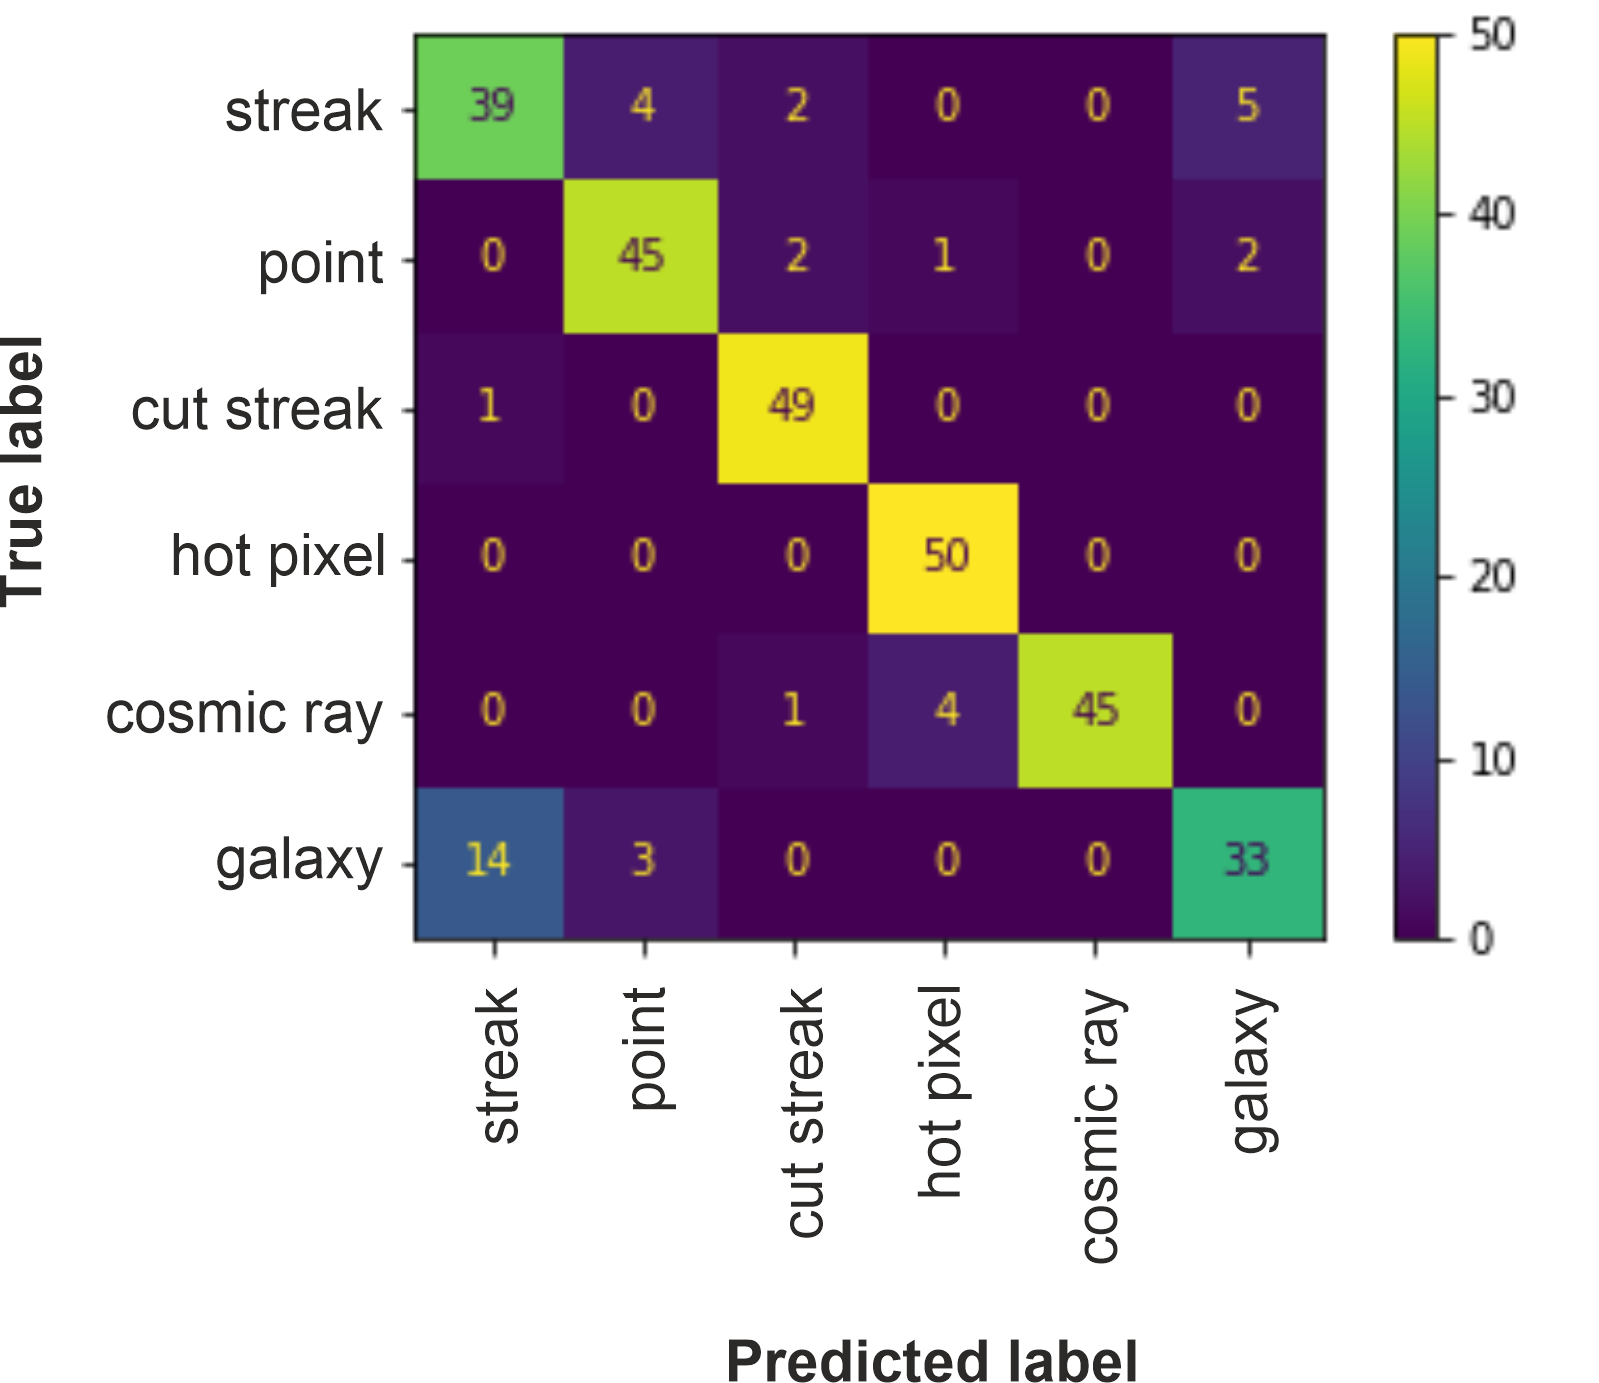
\includegraphics[width=.5\textwidth]{images/confusionMatrix13r_0.png}
    \caption{Confusion matrix from the testing of the model trained on merged synthetic and real data.}
    \label{img:confmatrixmerged}
\end{figure}

\begin{figure}[!h]
\centering
    \begin{subfigure}[t]{.23\textwidth}
        \centering
        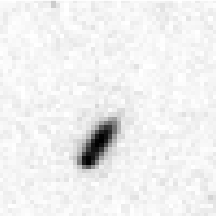
\includegraphics[width=\textwidth]{images/mwrongImage10.png}
        \caption{}
        \label{fig:galaxystreakmis2}
    \end{subfigure}
    \begin{subfigure}[t]{.23\textwidth}
        \centering
        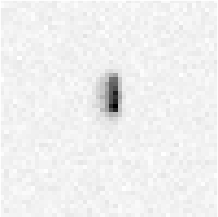
\includegraphics[width=\textwidth]{images/mwrongImage2.png}
        \caption{}
    \end{subfigure}
    \begin{subfigure}[t]{.23\textwidth}
        \centering
        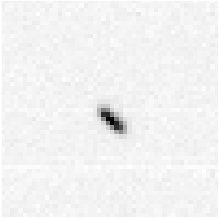
\includegraphics[width=\textwidth]{images/mwrongImage26.png}
        \caption{}
        \label{fig:streakpointmis2}
    \end{subfigure}
    \begin{subfigure}[t]{.23\textwidth}
        \centering
        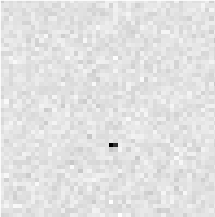
\includegraphics[width=\textwidth]{images/mwrongImage28.png}
        \caption{}
        \label{fig:cosmichotpixelmis}
    \end{subfigure}

    \caption[Wrongly classified images on the model that trained with merged synthetic and real data. ]
    {Wrongly classified images on the model that trained with merged synthetic and real data. (a) A galaxy misclassified as a streak, (b) A streak misclassified as a galaxy, (c) A streak misclassified as a point, (d) A cosmic ray misclassified as a hot pixel. }
    \label{fig:wrongmerged}
\end{figure}

\section{Model with fine-tuned fully-connected layers}
The model from Section \ref{subsec:fcmodel} has achieved the accuracy of 89.00 \%, precision of 89.19 \% and recall of 89 \% on the testing dataset. Of 300 images in the testing dataset, only 33 were wrongly classified. 

From the confusion matrix in the Figure \ref{img:confmatrixfc} we can see that the model is suffering from the same problems as the previous ones. This is mostly with the misclassification of streaks and galaxies (19 cases). Other problems are not that frequent and happen only in a few cases. Again, examples of some wrongly classified images are shown in the Figure \ref{fig:wrongfc}.
A point with a small fwhm has fewer pixels and is then misclassified as a cosmic ray (\ref{fig:pointcosmicmis}), while the other point which has a bigger fwhm is wrongly classified as a galaxy (\ref{fig:pointgalaxymis}). We can also see that even though the galaxy in the Figure \ref{fig:galaxylinemis} doesn't necessarily resembles a streak it is still classified as if it is. 

\begin{figure}[h]
    \centering
    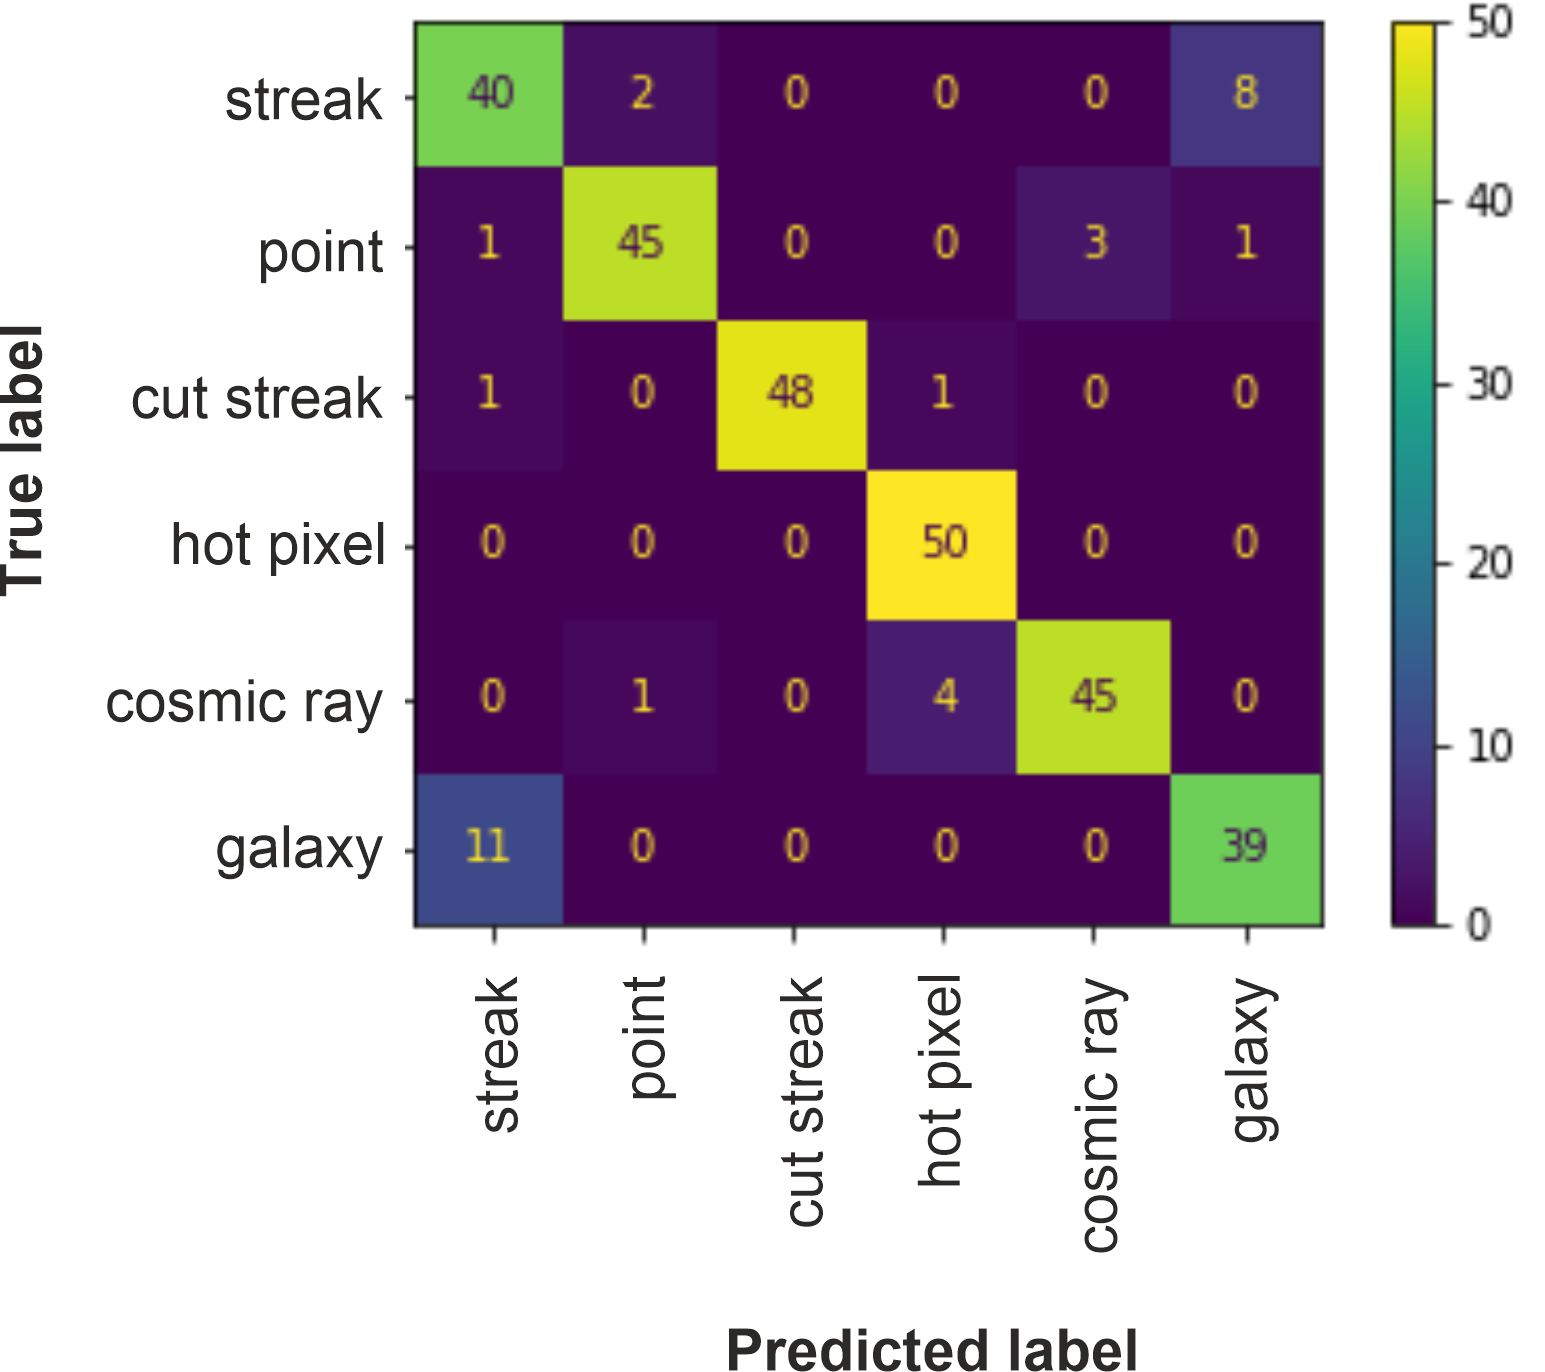
\includegraphics[width=.5\textwidth]{images/confusionMatrix14fe.png}
    \caption{Confusion matrix from the testing of the model with fine-tuned fully-connected layers.}
    \label{img:confmatrixfc}
\end{figure}

\begin{figure}[!h]
\centering
    \begin{subfigure}[t]{.23\textwidth}
        \centering
        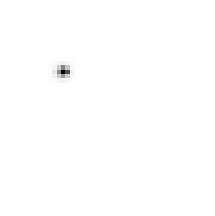
\includegraphics[width=\textwidth]{images/fcwrongImage1.png}
        \caption{}
        \label{fig:pointcosmicmis}
    \end{subfigure}
    \begin{subfigure}[t]{.23\textwidth}
        \centering
        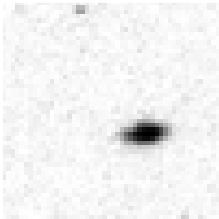
\includegraphics[width=\textwidth]{images/fcwrongImage3.png}
        \caption{}
        \label{fig:galaxylinemis}
    \end{subfigure}
    \begin{subfigure}[t]{.23\textwidth}
        \centering
        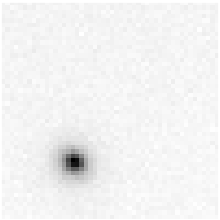
\includegraphics[width=\textwidth]{images/fcwrongImage10.png}
        \caption{}
        \label{fig:pointgalaxymis}
    \end{subfigure}
    \begin{subfigure}[t]{.23\textwidth}
        \centering
        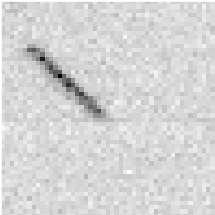
\includegraphics[width=\textwidth]{images/fcwrongImage21.png}
        \caption{}
    \end{subfigure}

    \caption[Wrongly classified images on the model with fine-tuned fully-connected layers.]
    {Wrongly classified images on the model with fine-tuned fully-connected layers. (a) A point misclassified as a cosmic ray, (b) A galaxy misclassified as a streak, (c) A point misclassified as a galaxy, (d) A streak misclassified as a galaxy. }
    \label{fig:wrongfc}
\end{figure}
\section{Summary}

The summary of all three models is depicted in the Table \ref{tab:summary}, which contains the accuracy, recall and precision on the testing dataset. In both fine-tuned models we can see a considerable improvement from the model that was trained only on the synthetic data. According to this, we can clearly state that the incorporation of the real data, even in such a small amount, has enhanced the capability of our model. 

If we compare the two fine-tuning approaches, they performed just slightly different. However fine-tuning only FC layers have achieved higher accuracy and training the model took significantly less time. One epoch of training all the layers on the whole merged training dataset took approximately 4 minutes. On the other hand, one epoch of tuning FC layers with the training dataset containing only real images took less than 30 seconds.

{\renewcommand{\arraystretch}{1.4}
\begin{table}[h]
\centering
\begin{tabular}{|l|c|c|c|}
\hline
\textbf{Model} & \multicolumn{1}{l|}{\textbf{Accuracy}} & \multicolumn{1}{l|}{\textbf{Precision}} & \multicolumn{1}{l|}{\textbf{Recall}} \\ \hline
\textit{\begin{tabular}[c]{@{}l@{}}model trained \\ on synthetic data\end{tabular}} & 73.00 \% & 73.52 \% & 73.00 \% \\ \hline
\textit{\begin{tabular}[c]{@{}l@{}}model trained\\ on merged data\end{tabular}} & 87.00 \% & 87.15 \% & 87.00 \% \\ \hline
\textit{\begin{tabular}[c]{@{}l@{}}model with fine-tuned \\ FC layers\end{tabular}} & 89.00 \% & 89.19 \% & 89.00 \% \\ \hline
\end{tabular}
\caption{A summary of the performance on the testing dataset on all three selected models. }
\label{tab:summary}
\end{table}
}
\section{ResNet}

To compare the performance of our model to state-of-the-art models, we have deployed ResNet-18 with following parameters: 
\begin{itemize}
    \item optimizer ADAM with the settings of $beta_1$ = 0.9 and $beta_2$ = 0.99
    \item learning rate of $1e^{-3}$
    \item L2 regularization with $\lambda$ of $1e^{-5}$
\end{itemize}


Training with only synthetic data, the ResNet-18 has achieved an accuracy of 69.33 \% on the testing dataset. Comparing this to our model, we have higher accuracy. However, this could be caused by the fact, that we have spent a lot of time tuning the hyperparameters on our network, but we haven't done the same with the ResNet. 

With incorporated real images into the training dataset, the ResNet has achieved an accuracy of 96 \%. In this case, the ResNet has surpassed our model, which is probably caused by the deeper architecture.  
